\documentclass[10pt]{beamer}
\usetheme{metropolis}

\usepackage{mathtools}
\usepackage{tikz}
\usetikzlibrary{shapes,arrows}
\usepackage[autosize]{dot2texi}
\usepackage{listings}

\title{Improving content discovery through combining linked data and data mining techniques}
\date{2016-05-16}
\author{Ross Fenning, Principal Software Engineer}
\institute{BBC Design and Engineering: Content Discovery}

\begin{document}
\maketitle

\begin{frame}[fragile]
\frametitle{Problem}
  \begin{columns}
    \begin{column}{0.5\textwidth}

    \begin{itemize}
        \item In the BBC, content is in multiple data stores
        \item \textgreater 10,000,000s of content items
        \item Content is diverse, systems are incompatible, etc.
    \end{itemize}

    \end{column}
    \begin{column}{0.5\textwidth}
      \centering
        \begin{dot2tex}[neato,scale=0.7]
            digraph g {
              rankdir=TB;

              A [label="News",shape="circle",color="red"];
              B [label="Video",shape="square",color="pink"];
              C [label="Audio",shape="box",color="pink"];
              D [label="Recipes",shape="triangle",color="green"];
              E [label="Sport Data",color="yellow"];

                Search -> A;
                Search -> B;
                Search -> C;
                Search -> D;
                Search -> E;

              }
        \end{dot2tex}
    \end{column}
  \end{columns}

  Cross-content functions like search, navigation, recommendations, etc. are difficult to implement.

  How can we learn enough about all our content and offer people links to interesting parts of the website they've not seen before?

\end{frame}

\begin{frame}[fragile]
\frametitle{Approach}

Data pipeline using semantics and linked data

    \begin{dot2tex}[dot,options=-t math,autosize,pgf,scale=0.45]
      digraph g {
        rankdir=LR;

        node [shape=circle,margin="0,0"]
        RDF1 [label="RDF_1"];
        RDF2 [label="RDF_2"];
        RDF3 [label="RDF_3"];
        RDFp [label="RDF'"];
        RDFp1 [label="RDF'_1"];

        IRI -> RDF1 [label="\text{parse}"];
        IRI -> RDF2 [label="\text{extract}"];
        IRI -> RDF3 [label="\text{scrape}"];

        RDF1 -> RDF [label="\cup"];
        RDF2 -> RDF [label="\cup"];
        RDF3 -> RDF [label="\cup"];

        RDF -> RDFp1 [label="\text{enrich}"];

        RDF -> RDFp [label="\cup"];
        RDFp1 -> RDFp [label="\cup"];

        RDFp -> Features [label="generate"];
      }
    \end{dot2tex}
    \begin{itemize}
        \item Construct RDF graphs from content items using linked data, entity extraction and more
        \item Enable or disable each and union each to get a single RDF graph
        \item Enrich that graph by extracting data about linked objects (other enrichment considered, but not implemented)
        \item Generate feature sets using SPARQL queries
        \item Apply clustering to feature sets
    \end{itemize}
\end{frame}

\begin{frame}
\frametitle{Outcomes}
  \begin{columns}
    \begin{column}{0.5\textwidth}

    \begin{center}

    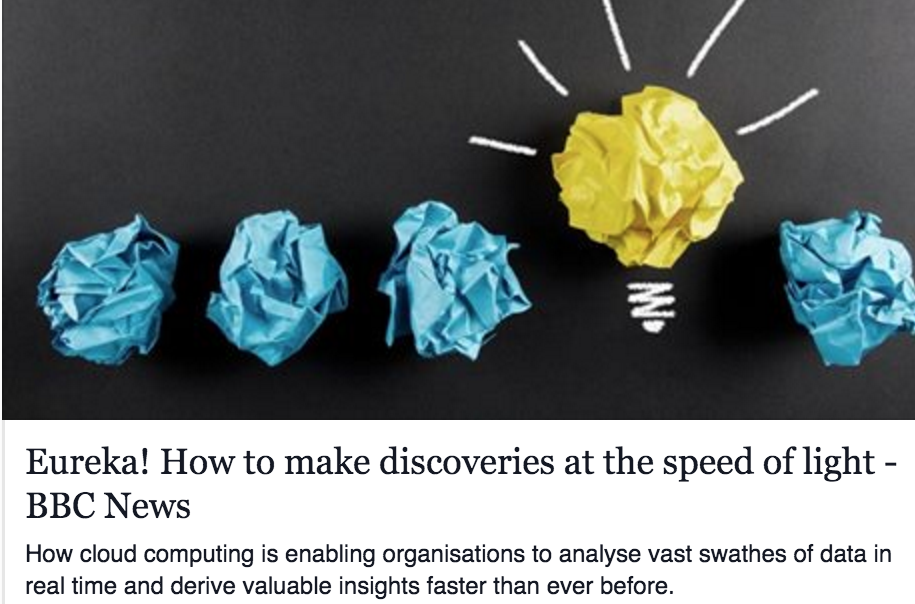
\includegraphics[height=2.9cm]{facebook.png}

    \vspace{0.5cm}

    \small
    Surveyed people preferred related
    content based on topics and themes. Entity extraction does this, but
    needs tuning.

    \end{center}

    \end{column}
    \begin{column}{0.5\textwidth}

    \begin{center}

        \small
        Extracting RDFa, etc. from the page finds basic categoriation
        for social media embedding. This article is from BBC News (technology news).

    \vspace{0.5cm}

        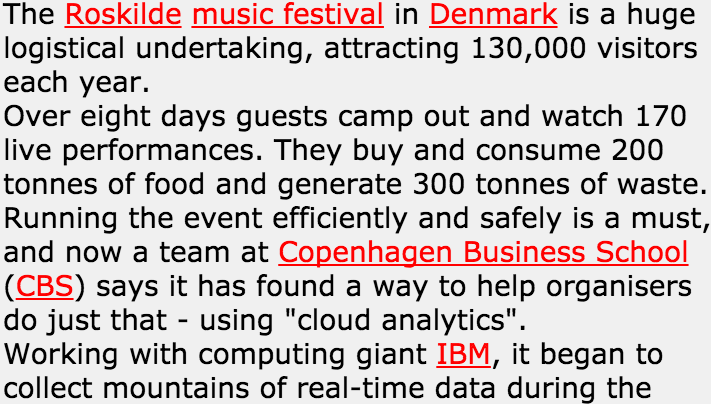
\includegraphics[height=2.9cm]{entities.png}
    \end{center}

    \end{column}
  \end{columns}

    \vspace{0.5cm}

Embedded semantics are trivial to extract, so start here.
Better clustering comes from combining with entity extraction,
if tuned.

Encrichment using embedded semantics of linked entities adds little.
Further research is needed for more sophisticated enrichment methods.

\end{frame}

\end{document}
